\documentclass[runningheads]{llncs}
\usepackage[utf8]{inputenc}
\usepackage{amsmath,amssymb}
\usepackage{graphicx}
\usepackage{booktabs,array}
\usepackage{url}
\usepackage[hidelinks]{hyperref}
\graphicspath{{../figs/}}
% Shared notation for the IEEE paper, the LNCS paper and the full report.
% Packages are loaded by each main.tex; this file only defines commands.
\providecommand{\QUBO}{QUBO}
\providecommand{\HUBO}{HUBO}
\newcommand{\Lam}{\ensuremath{\Lambda}}
\newcommand{\Lsafe}{\ensuremath{\Lambda_{\mathrm{safe}}}}
\newcommand{\Fset}{\ensuremath{\mathcal{F}}}
\newcommand{\Popt}{\ensuremath{P(\mathrm{opt})}}
\newcommand{\btrue}{\ensuremath{\mathrm{benefit}_{\mathrm{true}}}}
\newcommand{\Tstar}{\ensuremath{T^{\ast}}}
\newcommand{\Wstar}{\ensuremath{W^{\ast}}}
\newcommand{\degC}{\ensuremath{^{\circ}}C}
\newcommand{\gap}{\ensuremath{\Delta(s{=}1)}}
\newcommand{\code}[1]{\texttt{#1}}
\newcommand{\repo}{\texttt{s-siyanwal/q\_uhi}}
\newcommand{\sha}{\texttt{e649582}}
\newcommand{\blob}[1]{\url{https://github.com/s-siyanwal/q_uhi/blob/claude/clever-gates-ezote4/#1}}
% Unicode that appears in method names copied from the CSVs
\DeclareUnicodeCharacter{03B1}{\ensuremath{\alpha}}
\DeclareUnicodeCharacter{039B}{\ensuremath{\Lambda}}
\DeclareUnicodeCharacter{00B7}{\ensuremath{\cdot}}
\DeclareUnicodeCharacter{00D7}{\ensuremath{\times}}
\DeclareUnicodeCharacter{2264}{\ensuremath{\leq}}
\DeclareUnicodeCharacter{2265}{\ensuremath{\geq}}
\DeclareUnicodeCharacter{2212}{\ensuremath{-}}
\DeclareUnicodeCharacter{03BC}{\ensuremath{\mu}}
\DeclareUnicodeCharacter{2013}{--}
\DeclareUnicodeCharacter{2014}{---}
\DeclareUnicodeCharacter{2192}{\ensuremath{\rightarrow}}


\begin{document}
\title{Constraint Encodings, Not Annealers, Dominate QUBO/HUBO Siting for Urban Heat-Island Interventions}
\titlerunning{Constraint encodings dominate QUBO/HUBO siting for UHI}
\author{The \texttt{quhi} project}
\authorrunning{The \texttt{quhi} project}
\institute{Repository \repo{}, commit \sha}
\maketitle

\begin{abstract}
We site parks, water bodies and cool pavement on synthetic 50\,m city grids. Each instance is a
constrained binary program, encoded as a \QUBO{} or \HUBO{} and scored on exact saturating cooling
physics against a HiGHS-certified optimum. A slack-bit penalty \QUBO{} with a corrected weight has
the MILP optimum as its ground state on all 11 exhaustively enumerated instances. The second-order
Taylor \QUBO{} loses 10.3\% of the achievable cooling at 300\,m reach, where the cubic \HUBO{} loses
at most 0.02\% and a least-squares-fitted \QUBO{} at most 0.42\%. The final annealing gap scales as
$1/\Lam$ with the penalty weight. Constraint-preserving Dicke-XY QAOA reaches a mean $\Popt$ of
0.43 at depth 6, against 1.00 for feasible-space simulated annealing. Path-integral Monte Carlo
restricted to the feasible set passes a pre-committed comparability bar (benefit 0.981), but it
made 3.6$\times$ more proposals than feasible-space annealing; at equal proposals it scores 0.983
against 0.988. HiGHS certifies every hard-family instance in 0.77\,s on average. Encodings and
constraint handling, not the choice of annealer, decide the outcome. We observe no quantum or
quantum-inspired advantage.

\keywords{QUBO \and HUBO \and penalty encoding \and QAOA \and path-integral Monte Carlo \and urban heat island \and negative result}
\end{abstract}

%----------------------------------------------------------------------
\section{Introduction}\label{sec:intro}
This is a benchmarking study with a pre-registered bar and a negative outcome.
Quantum and quantum-inspired optimisers are often proposed for spatial planning problems that can
be written as \QUBO{}s. Urban-heat-island (UHI) mitigation is one such problem: choose where to put
parks, water bodies and cool pavement on a city grid, under a budget and an equity requirement, so
that the population-weighted air temperature is as low as possible. This work asks a narrow
question: \emph{on certified instances and at matched effort, does any quantum or quantum-inspired
method reach the benefit of the classical baselines?}

We answer it with a clean re-implementation, the \code{quhi} toolkit, after an audit found that an
earlier code base produced penalty artefacts rather than results
(Section~\ref{sec:audit}). Every plan is scored on the exact saturating cooling physics and
compared with a HiGHS-certified optimum~\cite{huangfu2018}. The success criterion was fixed in
advance: a method is at par only if, at matched wall-clock on certified instances, it meets the
greedy planner \emph{and} the MILP on both instance families. Matching simulated annealing is not
enough.

The answer is negative, and the reasons are specific. The encoding decides most of the outcome:
slack penalties set the annealing gap, Taylor truncation distorts long-reach cooling, and
quadratisation hides native higher-order structure. Once constraints are handled natively, a
feasible-space classical annealer is as good as the best quantum-inspired sampler we built, and
HiGHS certifies every hard instance in about a second.


\noindent\textbf{Contributions.} (i) A certified slack-penalty encoding with a bound about
$2\times$ tighter than the textbook one, verified exhaustively (E1). (ii) Evidence that surrogate
order and quadratisation, not the sampler, dominate solution quality (E2, E5, E11). (iii) A
depth curve for constraint-preserving QAOA against feasible-space SA (E8b). (iv) An equal-work
ablation showing that a feasible-space PIMC sampler's apparent lead is an artefact of extra
proposals (E12b).

%----------------------------------------------------------------------
\section{The Siting Problem}\label{sec:problem}
We keep the physics deliberately simple and the evaluation deliberately strict.
Following the Sanya green-space study~\cite{zhou2023}, a city is a grid of $50\times50$\,m cells
with fixed land uses. A decision variable $x_v\in\{0,1\}$, $v=(i,o)$, places option
$o\in\{\text{park},\text{water},\text{cool pavement}\}$ on candidate cell $i$. The cooling that
option $o$ at cell $i$ delivers to target cell $k$ is $e_{ik}=A_o\exp(-d_{ik}/L_o)$, with
illustrative defaults $A=1.5$\,\degC{}, $L=100$\,m (park), $A=2.0$\,\degC{}, $L=80$\,m (water) and
$A=0.6$\,\degC{}, $L=30$\,m (cool pavement), at costs of 3, 5 and 1 units.

\paragraph{Saturation.} Overlapping cool islands do not add without limit. We use
\begin{equation}
\Delta T_k(x)=\Delta T_{\max}\Bigl[1-\prod_v\bigl(1-p_{kv}x_v\bigr)\Bigr],\qquad
p_{kv}=\min(e_{kv},\Delta T_{\max})/\Delta T_{\max},
\label{eq:sat}
\end{equation}
with $\Delta T_{\max}=3$\,\degC{}. The objective is the exposure-weighted temperature
$f(x)=\sum_k w_k\bigl(T^0_k-\Delta T_k(x)\bigr)$, $w_k=0.7\,\mathrm{pop}_k/\sum\mathrm{pop}+0.3/N$.
Inclusion--exclusion truncated at order $K$ gives an additive model ($K{=}1$), a \QUBO{} ($K{=}2$)
or a cubic \HUBO{} ($K{=}3$). By the Bonferroni inequalities the \QUBO{} is a pessimistic bound on
the exact objective. An optional park-block synergy adds a quartic term for every complete
$2\times2$ block of parks.

\paragraph{Constraints.} An integer budget $\sum_v c_o x_v\le B$; at most one option per cell;
and, optionally, at least one intervention per district (equity). With one option per cell and no
equity, $-f$ is monotone submodular, so the cost-benefit greedy planner has a
$(1-1/e)$ guarantee~\cite{nemhauser1978}; any quantum claim must therefore beat greedy and MILP,
not only SA.

\paragraph{Scoring.} $\btrue$ is the exact-physics cooling of a returned plan divided by that of
the MILP plan; an infeasible plan scores 0. Because MILP certifies the $K{=}2$ surrogate and not
Eq.~\eqref{eq:sat}, $\btrue$ can slightly exceed 1. $\Popt$ is the fraction of runs (or the exact
probability, for QAOA) that return the certified optimum.


%----------------------------------------------------------------------
\section{A Cautionary Audit}\label{sec:audit}
Negative results are only credible if earlier positive-looking numbers are explained.
The repository started from an earlier code base and a set of design documents. The audit
(\code{docs/AUDIT.md}, reproduced by \code{scripts/audit\_legacy.py}) found that its results cannot be
used; 19 of its 163 tests fail. The findings that matter for this paper are:
\begin{itemize}
\item[F1] inequality constraints encoded as equalities in raw m$^2$, giving a coefficient ratio of
$1.72\times10^{9}$ against 2.0 and an infeasible global minimum;
\item[F2] shipped ``results'' whose energies are penalty magnitudes, with an all-zero SQA plan;
\item[F3] an SQA action with $\beta$ instead of $\beta/P$ on the problem term: the single-qubit
$\langle\sigma_z\rangle$ is $-0.997$ against the exact $-0.545$ (\code{quhi}: $-0.546$);
\item[F4] a penalty theorem that is false for non-integer data (the corrected bound is about
$2\times$ smaller, median ratio 2.06);
\item[F5] an automatic penalty weight that can be too small by a factor of $n$;
\item[F6] a \QUBO{}$\leftrightarrow$Ising round trip that doubles couplings;
\item[F7] worked examples and ``known optima'' that are wrong.
\end{itemize}
The legacy energies are artefacts of F1--F3 and are not cited anywhere in this work. The legacy
material also invoked asymptotic quantum-annealing results for one-dimensional disordered
chains~\cite{santoro2002}; those do not transfer to dense, penalty-dominated \QUBO{}s (E6).


\begin{table}[t]
\centering\caption{Legacy audit findings (from \texttt{docs/AUDIT.md}).}\label{tab:audit}
\scriptsize% typed from docs/AUDIT.md
\begin{tabular}{lp{0.36\linewidth}p{0.46\linewidth}}
\toprule
& finding & evidence (docs/AUDIT.md, results/audit/audit.json) \\
\midrule
F1 & inequalities encoded as equalities, in raw m$^2$ & $|Q|_{\max}=1.72\times10^{9}$ vs $|Q_{\text{phys}}|_{\max}=2.0$; infeasible global minimum \\
F2 & shipped ``results'' are artefacts & energies are penalty magnitudes; SQA returns the all-zero plan \\
F3 & SQA uses $\beta$ instead of $\beta/P$ & $\langle\sigma_z\rangle$: exact $-0.545$, \code{quhi} $-0.546$, legacy $-0.997$ \\
F4 & penalty theorem false for non-integer data & counter-example; corrected bound about $2\times$ smaller (median 2.06) \\
F5 & automatic penalty weight not a bound & too small by up to a factor $n$ ($Q=\mathbf{1}$, $n=10$: 10 vs 100) \\
F6 & \QUBO{}$\leftrightarrow$Ising round trip doubles couplings & round trip returns doubled off-diagonals \\
F7 & wrong worked examples and ``known optima'' & claimed $-19.25$ where $f=-5$ and the optimum is $-6$ \\
\bottomrule
\end{tabular}

\end{table}

%----------------------------------------------------------------------
\section{Encodings}\label{sec:enc}
Four encoding choices were tested before any quantum method was run.
\paragraph{Exact penalty (E1).} With integer constraint data and bounded binary slack bits, a
penalty weight $\Lam>f^\ast-L(f)$ is sufficient, where $f^\ast$ is the constrained optimum and
$L(f)$ any lower bound. Exhaustive enumeration of the full penalty \QUBO{} (decision plus slack
bits) on 11 instances shows that its ground state equals the MILP optimum on all 11
(Table~\ref{tab:e1}); $\Lsafe$ is 1.81--2.21$\times$ smaller than the range bound.

\paragraph{Penalty weight (E4).} On a mix $8\times8$ + equity instance, $0.01\,\Lsafe$ followed
by repair raises $\Popt$ after post-processing from at most 0.03 to 0.42 (SA) and 0.47 (Tabu).
Raw feasibility collapses below about $0.1\,\Lsafe$. The recipe is hybrid, not certified.

\paragraph{Penalty form (E10, quick run on 2 instances).} An unbalanced penalty at $0.1\,\Lsafe$
needs no slack bits (10 instead of 13 variables) and cuts the dynamic range from 163 to 16.5 with
the ground state still optimal on these instances. It is not certified in general, and the linear
(Lagrangian) form is feasible and optimal only for lucky multipliers.

\paragraph{Quadratisation (E11, quick run on 2 instances).} Rosenberg substitution
\cite{rosenberg1975,boros2002} of a cubic \HUBO{} leaves the slack-penalty final gap unchanged
($9.4\times10^{-5}$ and $1.1\times10^{-5}$) but adds 7 qubits (9 to 16) and lowers the short-anneal
ground-state probability from $3.1\times10^{-3}$ to $2.4\times10^{-5}$. Removing the penalty
altogether (a diagonal-only simulation on $\Fset$) enlarges the gap about 250$\times$.


\begin{table}[t]
\centering\caption{E1: penalty-\QUBO{} ground state versus MILP optimum on 11 exhaustively enumerated instances.}\label{tab:e1}
\resizebox{\textwidth}{!}{% generated by latex/tools/make_tables.py from results/ -- do not edit
\begin{tabular}{lrrrrcrr}
\toprule
instance & dec. & slack & MILP opt.\ (\degC) & QUBO ground (\degC) & match & $\Lambda_{\mathrm{safe}}$ & range/safe \\
\midrule
6x6\_s0\_park & 5 & 3 & 30.818 & 30.818 & yes & 1.906 & 1.881 \\
6x6\_s1\_park & 5 & 3 & 30.755 & 30.755 & yes & 1.825 & 1.839 \\
6x6\_s2\_park & 5 & 3 & 30.720 & 30.720 & yes & 1.845 & 1.854 \\
6x6\_s3\_park & 5 & 3 & 30.823 & 30.823 & yes & 2.045 & 1.815 \\
8x8\_s0\_park & 12 & 4 & 30.584 & 30.584 & yes & 2.961 & 2.124 \\
8x8\_s1\_park & 12 & 4 & 30.507 & 30.507 & yes & 2.330 & 2.208 \\
8x8\_s2\_park & 12 & 4 & 30.738 & 30.738 & yes & 2.417 & 2.193 \\
8x8\_s3\_park & 12 & 4 & 30.757 & 30.757 & yes & 2.706 & 2.146 \\
6x6\_s0\_mix & 15 & 3 & 30.369 & 30.369 & yes & 4.850 & 2.063 \\
6x6\_s1\_mix & 15 & 3 & 30.339 & 30.339 & yes & 4.538 & 2.018 \\
8x8\_s1\_park + equity & 12 & 11 & 30.552 & 30.552 & yes & 2.403 & 2.142 \\
\bottomrule
\end{tabular}
}
\end{table}

%----------------------------------------------------------------------
\section{Surrogates}\label{sec:sur}
How the saturating law is turned into a polynomial matters more than which sampler minimises it.
\paragraph{Truncation order (E2).} On $12\times12$ cities with 22 candidate cells and a park
budget of at most 6, each surrogate's optimum is found by enumerating all feasible plans and then
scored on Eq.~\eqref{eq:sat}. Table~\ref{tab:e2} gives the share of the achievable cooling lost.
At $L=300$\,m the Taylor \QUBO{} loses 10.30\%, because the second-order truncation over-counts
diminishing returns and spreads parks out. The cubic \HUBO{} loses at most 0.02\% at any $L$, and a
\QUBO{} with the same 253 coefficients fitted by least squares loses at most 0.42\%.

\paragraph{Native higher order (E5).} On a quartic \HUBO{} with 30 variables (cubic saturation
plus park-block synergy), Tabu search finds the certified optimum on 99.0\% of raw reads. After
Rosenberg quadratisation, which needs 187--197 variables, raw success drops to 0\%: the auxiliary
penalties create narrow valleys that single-flip dynamics cannot cross.


\begin{table}[t]
\centering\caption{E2: share of the achievable cooling lost by each surrogate's optimum, scored on the exact law.}\label{tab:e2}
\small% generated by latex/tools/make_tables.py from results/ -- do not edit
\begin{tabular}{rrrrr}
\toprule
$L$ (m) & additive $K{=}1$ & QUBO $K{=}2$ (Taylor) & QUBO (LSQ fit) & HUBO $K{=}3$ \\
\midrule
50 & 0.20\textbackslash\{\}\% & 0.00\textbackslash\{\}\% & 0.00\textbackslash\{\}\% & 0.00\textbackslash\{\}\% \\
100 & 0.00\textbackslash\{\}\% & 0.20\textbackslash\{\}\% & 0.02\textbackslash\{\}\% & 0.00\textbackslash\{\}\% \\
200 & 0.29\textbackslash\{\}\% & 2.81\textbackslash\{\}\% & 0.21\textbackslash\{\}\% & 0.02\textbackslash\{\}\% \\
300 & 0.00\textbackslash\{\}\% & 10.30\textbackslash\{\}\% & 0.42\textbackslash\{\}\% & 0.00\textbackslash\{\}\% \\
\bottomrule
\end{tabular}

\end{table}

%----------------------------------------------------------------------
\section{The Classical Bar}\label{sec:classical}
A quantum method has to beat these baselines, not only simulated annealing.
The classical bar consists of HiGHS~\cite{huangfu2018} on the constrained program, the
cost-benefit greedy planner, penalty-\QUBO{} SA~\cite{kirkpatrick1983} and
Tabu~\cite{glover1989}, and two feasible-space methods that never leave $\Fset$:
\emph{FeasibleSA} (Metropolis with add/remove and swap moves on $f$, no $\Lam$) and
\emph{Tabu-on-F}.

\paragraph{E3 (penalty QUBO, safe $\Lam$).} Tabu is the strongest sampler on single-intervention
\QUBO{}s ($\Popt=1.00$ up to 27 variables, 0.66 at 46). On the mix + equity family, no
penalty-\QUBO{} sampler reaches the optimum on raw reads. SQA's $+0.02$--$0.03$ benefit over
flip-matched SA costs about 2.4$\times$ the wall time.

\paragraph{Greedy.} The greedy planner is optimal on 8 of 15 park instances (worst gap
0.037\,\degC{}), but it ignores equity and is infeasible on 5 of 9 mix instances in E3 and on 6 of 9
family-H instances in E12.

\paragraph{E7 showcase.} On a $14\times14$ city with 81 decision variables, MILP certifies in
10.8\,s and lowers the exposure temperature from 32.311 to 31.141\,\degC{}; the greedy planner
returns the same plan.

\paragraph{HiGHS wall-clock.} 3.8\,s on average for the E9 mix + equity cities; 0.81\,s on
average (2.29\,s at most) for E12 family H; 0.77\,s on average in E12b; 1.67\,s for the E13 tile.
Certification slows above about 60 dense decision variables (a $20\times20$ pilot was not certified
in 120\,s).


\begin{table}[t]
\centering\caption{E3: median raw success per read on safe-penalty \QUBO{}s.}\label{tab:e3}
\resizebox{\textwidth}{!}{% generated by latex/tools/make_tables.py from results/ -- do not edit
\begin{tabular}{lrrrrrrr}
\toprule
family / vars & Greedy & SA & SA-matched & SQA & SQA-fixedT & Tabu & QAOA(p=4) \\
\midrule
park / 13 & 0.20 & 0.48 & 1.00 & 1.00 & 1.00 & 1.00 & 0.01 \\
park / 17 & 0.06 & 0.03 & 0.48 & 0.56 & 0.84 & 1.00 & -- \\
park / 27 & 0.00 & 0.00 & 0.00 & 0.00 & 0.00 & 1.00 & -- \\
park / 32 & 0.00 & 0.00 & 0.00 & 0.00 & 0.00 & 0.94 & -- \\
park / 46 & 0.00 & 0.00 & 0.00 & 0.00 & 0.00 & 0.66 & -- \\
mix+equity / 42 & 0.00 & 0.00 & 0.00 & 0.00 & 0.00 & 0.00 & -- \\
mix+equity / 56 & 0.00 & 0.00 & 0.00 & 0.00 & 0.00 & 0.00 & -- \\
mix+equity / 89 & 0.00 & 0.00 & 0.00 & 0.00 & 0.00 & 0.00 & -- \\
\bottomrule
\end{tabular}
}
\end{table}

%----------------------------------------------------------------------
\section{Gate-Model and Analog Simulations}\label{sec:quantum}
All quantum results in this paper are exact classical simulations of small systems.
\paragraph{Analog gap (E6).} On a 14-qubit instance (10 decision and 4 slack qubits) with
$H(s)=-(1-s)\sum X+sH_P$, the minimum gap sits at $s=1$ and scales as $1/\Lam$: $\gap=7.1\times10^{-5}$
at $0.1\,\Lsafe$ and $7.1\times10^{-7}$ at $10\,\Lsafe$, so the adiabatic scale
$1/\Delta^2$~\cite{albash2018} grows from $2.0\times10^{8}$ to $2.0\times10^{12}$. The
penalty, not the instance's classical hardness, sets the energy resolution. X-mixer
QAOA~\cite{farhi2014} at $p=6$ places only 0.17--0.19\% on the optimum; its approximation
ratio of about 0.998 is measured on a penalty-dominated scale and is cosmetic.

\paragraph{Constraint-preserving mixers (E8).} Dicke/XY and feasibility-projected
mixers~\cite{hadfield2019} keep the state in $\mathrm{span}(\Fset)$, so $P(\mathrm{feasible})=1$ by
construction, and $\Popt$ is 10--70$\times$ higher than X-mixer penalty QAOA at equal depth
(``exactly 3 parks'', $p=2$: 0.37 against 0.005). On mix + equity, XY-QAOA at $p=2$ reaches
$\Popt=0.003$ and benefit 0.61, against 0.39 and 0.92 for FeasibleSA.

\paragraph{Depth (E8b).} On three ``exactly 3 parks'' cities ($n=10$, $|\Fset|=120$), Dicke-XY
complete reaches a mean $\Popt$ of 0.427 at $p=6$ (range 0.17--0.65), against 1.000 for FeasibleSA
in 0.21\,s (Table~\ref{tab:e8b}, Fig.~\ref{fig:e8b}). Ring-XY at $p=6$ (0.111) is below complete-XY
at $p=1$ (0.134), and the X-mixer stays at uniform-over-$\Fset$ level (0.009 against 1/120).

\paragraph{What is simulated.} ConstrainedQAOA is an exact state-vector simulation on
$\mathrm{span}(\Fset)$ built from a dense $|\Fset|\times|\Fset|$ eigendecomposition; it is not a
compiled circuit, and its cost is a cost of the simulation.


\begin{table}[t]
\centering\caption{E6: 14-qubit final gap and QAOA optimum probability versus penalty weight.}\label{tab:e6}
\small% typed from docs/RESULTS.md (E6; source results/E6_quantum/quantum_small.csv)
\begin{tabular}{lcccc}
\toprule
$\Lam/\Lsafe$ & ground = opt. & $\gap$ & $1/\Delta^2$ & QAOA $\Popt$, $p{=}6$ \\
\midrule
0.1 & yes & $7.1\times10^{-5}$ & $2.0\times10^{8}$ & 0.0019 \\
0.3 & yes & $2.4\times10^{-5}$ & $1.8\times10^{9}$ & 0.0018 \\
1 & yes & $7.1\times10^{-6}$ & $2.0\times10^{10}$ & 0.0017 \\
3 & yes & $2.4\times10^{-6}$ & $1.8\times10^{11}$ & 0.0017 \\
10 & yes & $7.1\times10^{-7}$ & $2.0\times10^{12}$ & 0.0017 \\
\bottomrule
\end{tabular}

\end{table}

\begin{table}[t]
\centering\caption{E8b: exact $\Popt$ versus depth, mean [min--max] over three ``exactly 3 parks'' cities, with classical references.}\label{tab:e8b}
\resizebox{\textwidth}{!}{% generated by latex/tools/make_tables.py from results/ -- do not edit
\begin{tabular}{lrrrrr}
\toprule
method & $p{=}1$ & $p{=}2$ & $p{=}3$ & $p{=}4$ & $p{=}6$ \\
\midrule
Dicke-XY complete & 0.134 & 0.242 [0.08--0.37] & 0.309 & 0.376 & 0.427 [0.17--0.65] \\
Dicke-XY ring & 0.034 & 0.067 [0.02--0.14] & 0.057 & 0.066 & 0.111 [0.02--0.26] \\
X-mixer penalty QAOA & 0.004 & 0.005 & 0.006 & 0.008 & 0.009 \\
\bottomrule
\end{tabular}
}\\[6pt]
\small% generated by latex/tools/make_tables.py from results/ -- do not edit
\begin{tabular}{lrrr}
\toprule
method & \Popt & benefit & wall (s) \\
\midrule
MILP (HiGHS) & 1.000 & 1.000 & 0.317 \\
Greedy planner & 0.667 & 1.000 & $8.54\times10^{-4}$ \\
uniform on F & 0.008 & 0.849 & 0.000 \\
FeasibleSA & 1.000 & 1.000 & 0.206 \\
\bottomrule
\end{tabular}

\end{table}

\begin{figure}[t]
\centering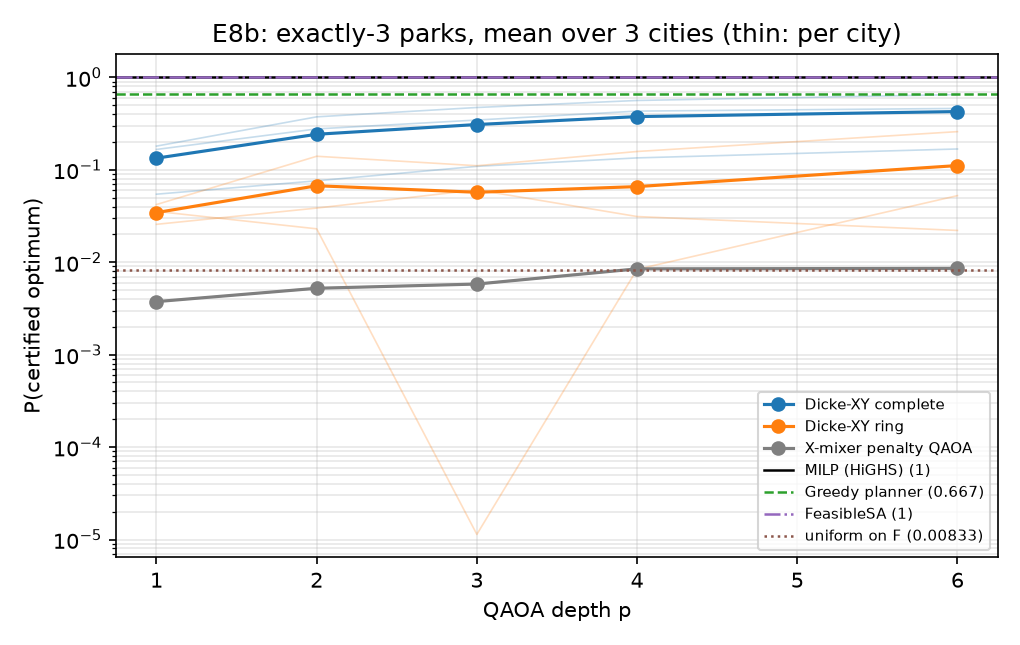
\includegraphics[width=0.7\textwidth]{p_opt_vs_p.png}
\caption{E8b: $\Popt$ versus QAOA depth for complete and ring Dicke-XY mixers and the X-mixer penalty control.}\label{fig:e8b}
\end{figure}

%----------------------------------------------------------------------
\section{Feasible-Space Path-Integral Monte Carlo}\label{sec:pimc}
The strongest quantum-inspired candidate is also the one whose result needs the most careful
accounting.
\paragraph{FeasibleSQA.} Path-integral Monte Carlo~\cite{martonak2002} with $P=8$ Trotter slices,
each a feasible plan, samples
$\pi(X)\propto\exp\bigl(-\tfrac{\beta}{P}\sum_k f(x^k)+J\sum_{k,i}s^k_is^{k+1}_i\bigr)$ with
$J=\tfrac12\ln\coth(\beta\Gamma/P)$, using the FeasibleSA moves on one slice at a time. It
reproduces the exact single-qubit $\langle\sigma_z\rangle$ and is quantum-\emph{inspired}: no
annealer implements a transverse field restricted to $\Fset$~\cite{heim2015}.

\paragraph{E12: matched wall-clock.} Family H has 9 instances ($8\times8$, $10\times10$,
$12\times12$ cities, seeds 100--102) with three intervention types, budget equal to the grid side,
equity, and a quartic synergy on the two larger sizes. Each method gets $\Tstar$ per run, the
larger of default FeasibleSA's median wall-clock and HiGHS's (capped at 8\,s). The pre-committed
COMPARABLE rule requires $P(\mathrm{feas})=1$, a family-mean benefit of at least 0.95$\times$ the
best classical mean, and no run over $1.5\,\Tstar$. FeasibleSQA passes with 0.981
(Table~\ref{tab:e12}), but FeasibleSA (0.973) and Tabu-on-F (0.976) pass the same bar, MILP reaches
1.000 in 0.81\,s, and the QAOA contestants do not qualify.

\paragraph{E12b: the ablation.} HiGHS was faster than default FeasibleSA on every instance, so
E12's $\Tstar$ was FeasibleSA's own time and there was no padding. The difference was work:
FeasibleSQA rejects moves that would leave $\Fset$ before evaluating $f$, so in the same wall-clock
it made 3.6$\times$ as many proposals (4.66\,M against 1.30\,M per run). Giving every method the
same proposal budget $\Wstar$ (4.53\,M per run on average) reverses the order: FeasibleSA 0.988,
FeasibleSQA 0.983, Tabu-on-F 0.977 (Table~\ref{tab:e12b}). FeasibleSQA stays within 5\% of
FeasibleSA (it is ahead on 1 instance, tied on 6, behind on 2) but does not beat it. E12 must not be
cited as a quantum-inspired win.


\begin{table}[t]
\centering\caption{E12: family H at matched wall-clock $\Tstar$ (pre-committed COMPARABLE rule).}\label{tab:e12}
\resizebox{\textwidth}{!}{% generated by latex/tools/make_tables.py from results/ -- do not edit
\begin{tabular}{lrrrrrc}
\toprule
method (family H) & P(feas) & \Popt & benefit & min & wall (s) & comp. \\
\midrule
MILP (HiGHS, 8 s cap) & 1.000 & 1.000 & 1.000 & 1.000 & 0.809 & yes \\
Greedy planner & 0.333 & 0.333 & 0.333 & 0.000 & 0.009 & no \\
FeasibleSA & 1.000 & 0.778 & 0.973 & 0.813 & 7.693 & yes \\
Tabu-on-F & 1.000 & 0.778 & 0.976 & 0.708 & 8.120 & yes \\
SA-matched α=0.01 + repair & 0.833 & 0.722 & 0.831 & 0.000 & 7.847 & no \\
FeasibleSQA & 1.000 & 0.722 & 0.981 & 0.854 & 7.975 & yes \\
QAOA-seeded FeasibleSA & 1.000 & 0.833 & 0.873 & 0.000 & 8.095 & no \\
ConstrainedQAOA p=2 & 1.000 & 0.500 & 0.658 & 0.000 & 2.008 & no \\
ConstrainedQAOA p=4 & 1.000 & 0.167 & 0.665 & 0.000 & 2.221 & no \\
\bottomrule
\end{tabular}
}
\end{table}

\begin{table}[t]
\centering\caption{E12b: family H on the tight clock and at equal proposals $\Wstar$. ``$\geq$0.95 FSA'' and ``beats'' compare with FeasibleSA on the same clock and instances.}\label{tab:e12b}
\resizebox{\textwidth}{!}{% generated by latex/tools/make_tables.py from results/ -- do not edit
\begin{tabular}{llrrrrrccc}
\toprule
method & clock & \Popt & benefit & min & wall (s) & prop.\ (M) & $\geq$0.95 FSA & beats & w/t/l \\
\midrule
MILP (HiGHS, 8 s cap) & none & 1.000 & 1.000 & 1.000 & 0.77 & -- & -- & -- & -- \\
FeasibleSA & tight & 0.778 & 0.973 & 0.813 & 7.13 & 1.30 & yes & no & -- \\
Tabu-on-F & tight & 0.833 & 0.977 & 0.708 & 7.45 & 2.96 & yes & yes & 2/5/2 \\
FeasibleSQA & tight & 0.722 & 0.981 & 0.854 & 7.42 & 4.66 & yes & yes & 3/6/0 \\
QAOA-seeded FeasibleSA & tight & 1.000 & 0.667 & 0.000 & 2.07 & 0.18 & no & no & 0/2/1 \\
FeasibleSA & equal\_work & 0.889 & 0.988 & 0.854 & 24.99 & 4.53 & yes & no & -- \\
Tabu-on-F & equal\_work & 0.833 & 0.977 & 0.708 & 11.32 & 4.65 & yes & no & 1/6/2 \\
FeasibleSQA & equal\_work & 0.778 & 0.983 & 0.813 & 7.09 & 4.53 & yes & no & 1/6/2 \\
QAOA-seeded FeasibleSA & equal\_work & 1.000 & 1.000 & 1.000 & 2.28 & 2.20 & yes & no & 0/3/0 \\
\bottomrule
\end{tabular}
}
\end{table}

\begin{figure}[t]
\centering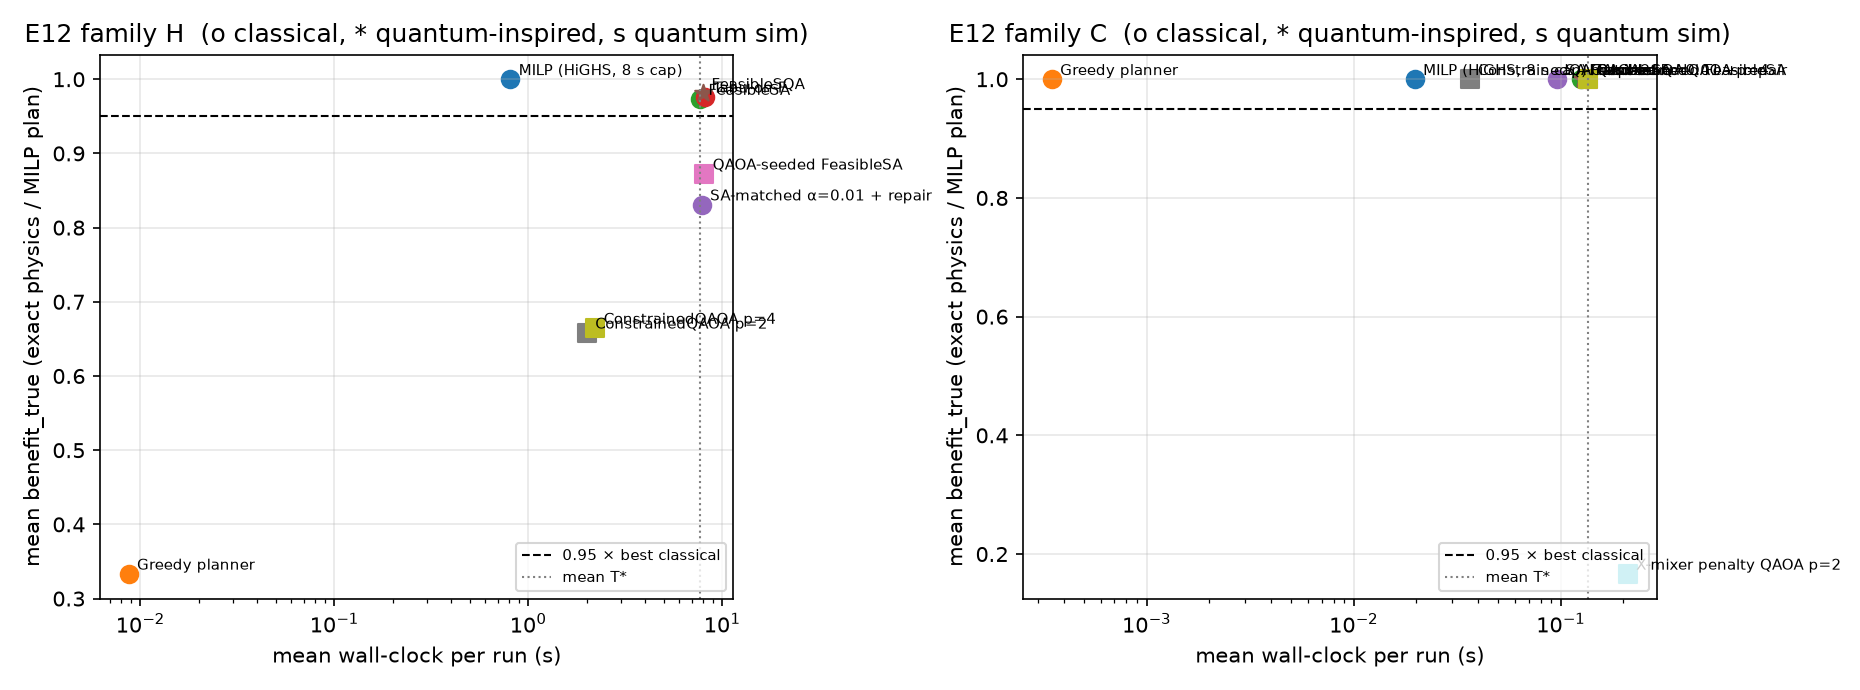
\includegraphics[width=\textwidth]{e12_benefit_vs_time.png}
\caption{E12: mean $\btrue$ versus mean wall-clock per run; dashed line: 0.95 of the best classical mean.}\label{fig:e12}
\end{figure}

%----------------------------------------------------------------------
\section{A Land-Surface-Temperature-Shaped Tile}\label{sec:tile}
Finally we tried to construct a case where the classical solver would struggle.
E13 builds one land-surface-temperature-shaped $16\times16$ tile: a compact hot core with a cool
edge, population concentrated on the core, and only 2 candidate lots left inside the core. With
three intervention types, equity and a budget of 16 it has $n=108$ and $|\Fset|>4000$, so
ConstrainedQAOA cannot be simulated. At a tight clock of 68.59\,s per run (Table~\ref{tab:e13}),
HiGHS certifies the tile in 1.67\,s and the greedy planner is infeasible on equity, the same failure
as on family H. The weak-penalty hybrid ($0.01\,\Lsafe$ + repair) finds the optimum on both seeds,
FeasibleSQA averages 0.9998 and FeasibleSA 0.9569 on two seeds each; by E12b a tight-clock
comparison hands FeasibleSQA several times more proposals, so this gap is not evidence of an
advantage. The mask created no classical gap.


\begin{table}[t]
\centering\caption{E13: $16\times16$ LST-shaped tile, tight clock, two sampler seeds.}\label{tab:e13}
\small% generated by latex/tools/make_tables.py from results/ -- do not edit
\begin{tabular}{lrrrr}
\toprule
method & P(feas) & \Popt & benefit & wall (s) \\
\midrule
MILP (HiGHS, 8 s cap) & 1.0 & 1.0 & 1.0000 & 1.67 \\
Greedy planner & 0.0 & 0.0 & 0.0000 & 0.06 \\
FeasibleSA & 1.0 & 0.5 & 0.9569 & 66.56 \\
Tabu-on-F & 1.0 & 0.0 & 0.6412 & 67.35 \\
FeasibleSQA & 1.0 & 0.5 & 0.9998 & 63.72 \\
SA-matched α=0.01 + repair & 1.0 & 1.0 & 1.0000 & 64.68 \\
\bottomrule
\end{tabular}

\end{table}

\begin{figure}[t]
\centering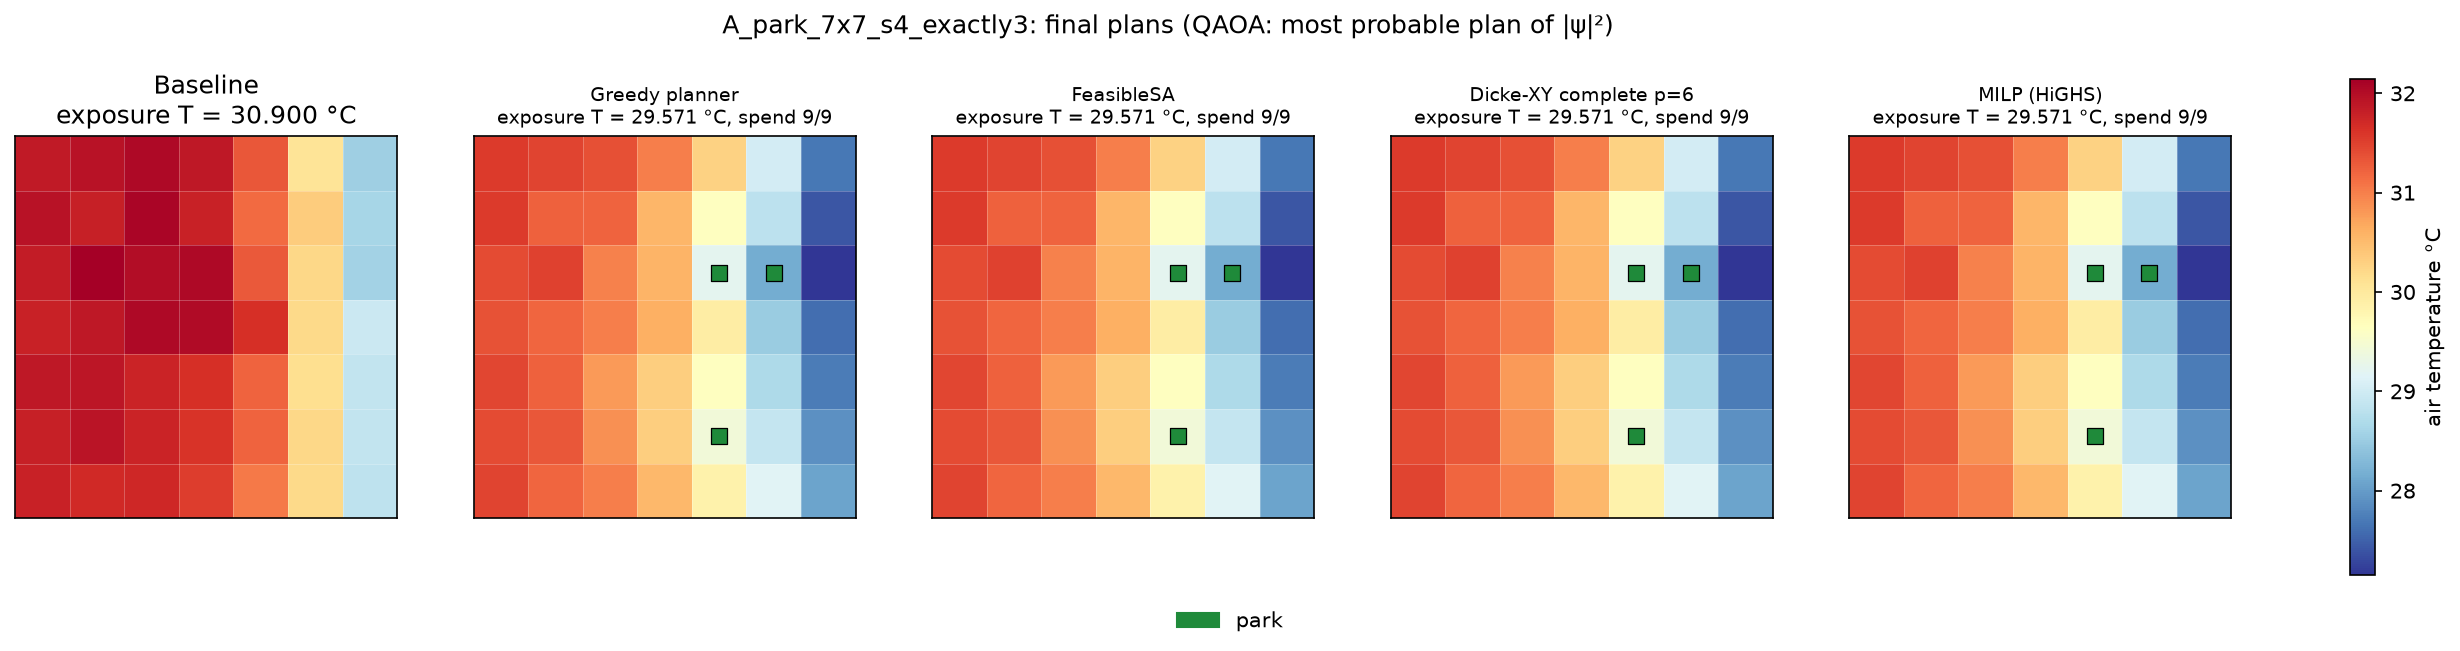
\includegraphics[width=\textwidth]{compare_final.png}
\caption{Final plans on the E8b ``exactly 3 parks'' city (greedy, FeasibleSA, Dicke-XY $p=6$ most probable plan, MILP). Animated versions: \texttt{results/ANIM/compare\_temp\_*.gif}.}\label{fig:anim}
\end{figure}

%----------------------------------------------------------------------
\section{Discussion}\label{sec:discussion}
\paragraph{Success criterion.} The criterion of Section~\ref{sec:intro} is not met by gate-model
QAOA: with penalties it learns the constraint rather than the objective (E6, E8b), and with
constraint-preserving mixers it remains well below FeasibleSA and MILP at every depth we simulated
(E8, E8b, E12). Feasible-space PIMC meets a 0.95 bar relative to the best classical method, but it
only ties feasible-space SA, and at equal proposals it is slightly behind (E12b).

\paragraph{What decided the outcome.} Each step that improved a quantum or quantum-inspired method
was a change of \emph{encoding}: certified but gentler penalties (E1, E4, E10), native higher-order
terms instead of quadratisation (E5, E11), and moves or mixers that respect the constraints (E8,
E12). Each of those changes helped the classical methods at least as much. The objective's
submodularity makes greedy strong wherever equity does not bind, and HiGHS certifies every
benchmark instance quickly.

\paragraph{What hardware could still test.} A fair hardware test would submit the constrained
model natively, as a CQM to a hybrid solver, on the E8b ``exactly 3'' city (seed 4) and a family-C
park city (seed 100). A safe-$\Lam$ slack \QUBO{} should never be sent to a QPU, because its gap is
set by $\Lam$ (E6, E11). The repository contains a hook that is inactive without an API token; no
D-Wave result exists.


\section{Limitations}\label{sec:limitations}
\begin{itemize}
\item \textbf{Synthetic cities.} All cities and the E13 tile are synthetic; no Landsat LST or census
layers were used, and intervention amplitudes and decay lengths are illustrative.
\item \textbf{Surrogate physics.} The saturation law stands in for CFD or ENVI-met; MILP certifies the
$K{=}2$ surrogate, not the exact physics.
\item \textbf{PIMC $\neq$ QPU.} SQA and FeasibleSQA are classical Monte Carlo samplers~\cite{heim2015}.
\item \textbf{Simulated circuits.} ConstrainedQAOA is a subspace simulation on $\mathrm{span}(\Fset)$,
not a compiled circuit, and X-mixer QAOA is limited to $\le16$ qubits.
\item \textbf{No hardware numbers.} No D-Wave, Leap or other cloud result is reported.
\item \textbf{Small samples.} Three instances $\times$ two seeds per E12/E12b cell; E10 and E11 are quick
runs on two instances.
\end{itemize}


\subsubsection*{Acknowledgements.}
{\sloppy
The experiments, the toolkit and this manuscript were produced in the \repo{} repository
(branch \code{claude/clever-gates-ezote4}, commit \sha). No external data, cloud solver or
quantum hardware was used.\par}


\bibliographystyle{splncs04}
\bibliography{../bib/refs}
\end{document}
